\documentclass[fontsize=11pt, paper=a4, titlepage=false]{scrartcl}


% geometry: change margins
% floatrow: customize layout of floating environments
% graphicx: include images
\usepackage[margin=2.2cm]{geometry}
\usepackage[margins=centering, objectset=centering]{floatrow}
\usepackage{graphicx}


% inputenc: support for writing UTF-encoded characters (accents, etc.)
% fix-cm: use default (OT1) font sizes (in conjunction with T1 fontenc)
% lmodern: latin modern font
% fontenc: better font encoding than default ascii
\usepackage[utf8]{inputenc}
\usepackage{fix-cm}
\usepackage{lmodern}
\usepackage[T1]{fontenc}


% babel: English hyphenation
% super: Lazy superscripting of countables
\usepackage[english]{babel}
\usepackage[super]{nth}


% todonotes: include todos
\usepackage{todonotes}


% authblk: Author affiliation options
\usepackage{authblk}
\renewcommand\Affilfont{\itshape\small}


% biblatex: bibliography
% csquotes: context sensitive quotation for BibLaTeX
\usepackage[backend=bibtex, bibencoding=inputenc, style=numeric-comp, 
sorting=none, hyperref=auto, isbn=false, doi=false, maxbibnames=100, 
minbibnames=100, url=false, giveninits=true, terseinits=true]{biblatex}
\addbibresource{bib.bib}
\DeclareNameAlias{sortname}{family-given}
\DeclareNameAlias{default}{family-given}
\renewcommand*{\revsdnamepunct}{}
\renewcommand*{\finalnamedelim}{\addcomma\addspace}
\DeclareFieldFormat*{citetitle}{#1}
\DeclareFieldFormat*{title}{#1}
\DeclareFieldFormat*{journaltitle}{#1}
\renewbibmacro{in:}{}
\AtEveryBibitem{\clearfield{month}}
\AtEveryBibitem{\clearfield{day}}
\renewbibmacro*{journal+issuetitle}{%
  \usebibmacro{journal}%
  \setunit*{\addspace}%
  \iffieldundef{series}
    {}
    {\newunit
     \printfield{series}%
     \setunit{\addspace}}%
  \usebibmacro{issue+date}%
  \setunit{\addsemicolon}%
  \usebibmacro{volume+number+eid}% 
  \setunit{\addsemicolon}%
  \usebibmacro{issue}%
  \newunit}
\newbibmacro*{issue+date}{%
    \iffieldundef{issue}
      {\usebibmacro{date}}
      {\printfield{issue}%
       \setunit*{\addspace}%
       \usebibmacro{date}}%
  \newunit}
\renewcommand*{\bibpagespunct}{\addcolon}
\DeclareFieldFormat{pages}{#1}
\usepackage{csquotes}

% enumitem: inline lists
\usepackage[inline]{enumitem}

% lineno: line numbers in margin
\usepackage{lineno}
\linenumbers

% hyperref: clickable links
% cleveref: better references
% glossaries: acronyms and glossaries
\usepackage[breaklinks=true, hidelinks=true]{hyperref}
\usepackage[noabbrev]{cleveref}
\usepackage[acronym, nogroupskip, nomain, nonumberlist, nopostdot, shortcuts, 
toc]{glossaries}
\setacronymstyle{long-short}


% suppres warnings about PDF page groups
\pdfsuppresswarningpagegroup=1


% set caption style
\setkomafont{caption}{\small}
\setkomafont{captionlabel}{\bfseries}
\setcapindent{0pt}


% pdf metadata
\hypersetup{
pdftitle = {Proceedings of the EuBIC Developer's Meeting 2018},
pdfauthor = {Wout Bittremieux}
}


% title and authors
\title{Proceedings of the EuBIC Developer's Meeting 2018}

\author[1]{Sander Willems}
\author[2]{David Bouyssi\'e}
\author[1]{Dieter Deforce}
\author[3]{Viktoria Dorfer}
\author[4]{Vladimir Gorshkov}
\author[5]{Dominik Kopczynski}
\author[6]{Kris Laukens}
\author[2]{Marie Locard-Paulet}
\author[4]{Veit Schw\"ammle}
\author[7]{Julian Uszkoreit}
\author[8,9]{Dirk Valkenborg}
\author[10,11]{Marc Vaudel}
\author[6,12]{Wout Bittremieux}

\affil[1]{Laboratory of Pharmaceutical Biotechnology, Ghent University, Ghent, 
Belgium}
\affil[2]{Institute of Pharmacology and Structural Biology, University of 
Toulouse, CNRS, UPS, Toulouse, France}
\affil[3]{Bioinformatics Research Group, University of Applied Sciences Upper 
Austria, Hagenberg, Austria}
\affil[4]{Department of Biochemistry and Molecular Biology, University of 
Southern Denmark, Odense M, Denmark}
\affil[5]{Leibniz-Institut für Analytische Wissenschaften -- ISAS -- e.V., 
Dortmund, Germany}
\affil[6]{Department of Mathematics and Computer Science, University of 
Antwerp, Antwerp, Belgium}
\affil[7]{Medizinisches Proteom-Center, Ruhr University Bochum, Bochum, Germany}
\affil[8]{Interuniversity Institute for Biostatistics and Statistical 
Bioinformatics, Hasselt University, Hasselt, Belgium}
\affil[9]{Centre for Proteomics, University of Antwerp, Antwerp, Belgium}
\affil[10]{KG Jebsen Center for Diabetes Research, Department of Clinical 
Science, University of Bergen, Bergen, Norway}
\affil[11]{Center for Medical Genetics and Molecular Medicine, Haukeland 
University Hospital, Bergen, Norway}
\affil[12]{Department of Genome Sciences, University of Washington, Seattle WA, 
USA}

\date{}


% acronyms
\newacronym{api}{API}{application programming interface}
\newacronym{dia}{DIA}{data-independent acquisition}
\newacronym{eubic}{EuBIC}{European Bioinformatics Community}
\newacronym{eupa}{EuPA}{European Proteomics Association}
\newacronym{lfq}{LFQ}{label-free quantification}
\newacronym{oms}{OMS}{open modification searching}
\newacronym{ptm}{PTM}{post-translational modification}
\newacronym{qc}{QC}{quality control}
\newacronym{ms}{MS}{mass spectrometry}
\newacronym{fwo}{FWO}{Research Foundation -- Flanders}
\newacronym{pca}{PCA}{principal component analysis}
\newacronym{ojo}{OJO}{Framework for Young Researchers}
\newacronym{bepa}{BePA}{Belgian Proteomics Association}
\newacronym{sib}{SIB}{Swiss Institute of Bioinformatics}

\begin{document}

\maketitle

\begin{abstract}
The inaugural \gls{eubic} developer's meeting was held from January \nth{9} to 
January \nth{12} 2018 in Ghent, Belgium.
While the meeting kicked off with an interactive keynote session featuring four 
internationally renowned experts in the field of computational proteomics, its 
primary focus were the hands-on hackathon sessions which featured six 
community-proposed projects revolving around three major topics:
\begin{enumerate*}[label=(\roman*),itemjoin={{; }},itemjoin*={{; 
and }},afterlabel=\unskip{{~}}]
\item quality control
\item workflows, protocols, and guidelines
\item quantification.
\end{enumerate*}
Here, we present an overview of the scientific program of the \gls{eubic} 
developer's meeting and provide a starting point for follow-up on the covered 
projects.
\end{abstract}

\glsresetall

\section{Introduction}

The \gls{eubic} is an initiative of the \gls{eupa} to promote the use of 
bioinformatics for computational \gls{ms} and \gls{ms}-based proteomics. Our 
goal is to bring together the European \gls{ms} bioinformatics community, 
including students and early-career researchers as well as long-standing 
experts from both academia and industry. Through the setup of community-driven 
dynamics, \gls{eubic} mainly focuses on improving education in computational 
methods, job and funding opportunities, international 
collaborations, publication of specialized studies, and training of software 
tools.
To this end, \gls{eubic} maintains several web resources that include 
educational videos, grant overviews, a job fair, and tutorials 
(\url{https://www.proteomics-academy.org/}). Besides these online resources, 
\gls{eubic} regularly organizes workshops and hubs at the major international 
conferences on computational \gls{ms} and proteomics. Additionally, an annual 
conference on computational \gls{ms}-based proteomics is organized by 
\gls{eubic} itself, forming an important community outreach effort to bring 
together bioinformatics researchers from all over Europe.

The first \gls{eubic} conference took place in January 2017 in Semmering, 
Austria~\autocite{Willems2017}. As this turned out to be an overwhelming 
success, we envisioned to organize the \gls{eubic} conference as an annual 
series. However, although this event brought together the European proteomics community, we observed that not all computational expertise was utilized to its full potential in the typical conference setup consisting of presentations and workshops. Therefore we 
decided to alternate the annual \gls{eubic} conference between a Winter School 
targeting a broad end user-oriented audience and a developer's meeting for 
software developers. 

The inaugural \gls{eubic} developer's meeting was organized in Ghent, Belgium, 
from January \nth{9} to January \nth{12} 2018 
(\url{http://uahost.uantwerpen.be/eubic18/}). A total of 43 participants 
(\cref{fig:group_foto}), including students, keynote speakers, and industry 
representatives from 14 different countries participated in the developer's 
meeting. To stimulate direct collaboration and the active development of 
bioinformatics applications, its main activity was a hackathon focusing on six 
important topics in computational proteomics which were crowd-sourced from the 
community. Additionally, prior to these hackathon sessions the meeting 
participants engaged in an interactive keynote session led by four 
internationally renowned scientists with experience in tool development for 
\gls{ms}-based proteomics.

\begin{figure}[!h]
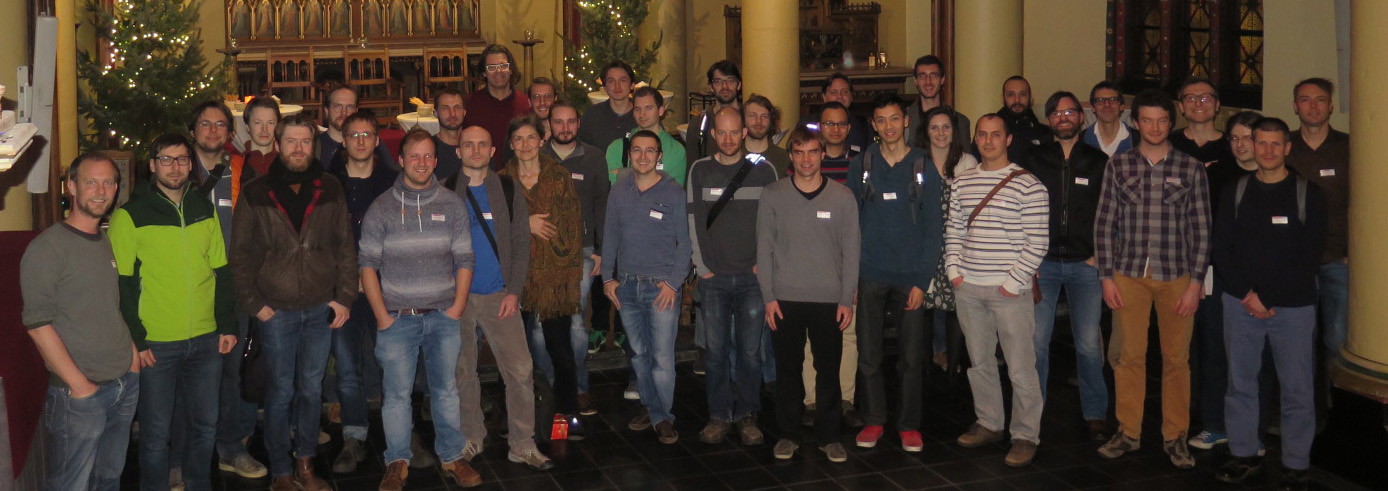
\includegraphics[width=\textwidth]{group_foto_eubic}
\caption{Participants of the \gls{eubic} developer's meeting 2018.}
\label{fig:group_foto}
\end{figure}

\section{Keynote presentations}

The \gls{eubic} developer's meeting kicked off with four keynote presentations 
illustrating some important current drawbacks of \gls{ms}-based data analysis 
and the crucial role of bioinformatics in solving these outstanding issues.

Prof.~dr.~Lennart Martens of Ghent University, Belgium, opened the meeting by 
describing his vision on the role of a bioinformatics scientist as a 
``researcher-developer''. As life sciences research has accelerated enormously 
over the past two decades, nowadays it is heavily dominated by the huge amount 
of data that are generated and the advanced algorithmic techniques that are 
necessary to analyze these data. He outlined that the job of a 
researcher-developer is to use and develop sophisticated algorithms and 
powerful tools to increase our understanding of the sheer complexity of 
biological systems~\autocite{Martens2015}. This was followed by an interactive 
discussion on career aspects and the growth path of bioinformatics researchers.

Next, dr.~Fr\'ed\'erique Lisacek of the \gls{sib}, 
Switzerland, presented her work on bridging proteomics and glycomics. She 
described difficulties prohibiting the fully automated identification of 
glycoproteomics data and explained how her group has tackled some of these 
issues. By making use of \glsentrylong{oms} peptides with previously 
unconsidered \glspl{ptm} could be successfully 
identified~\autocite{Horlacher2016}. Next, she explained how new computational 
tools can be used for the analysis of glycoproteomics 
data~\autocite{Horlacher2017}.

The third keynote speaker was dr.~Laurent Gatto of the University of Cambridge, 
England, who gave a presentation on the ecosystem of open-source tools in the R 
programming language for the analysis of \gls{ms} data~\autocite{Gatto2014}. 
Dr.~Gatto showed a historical perspective on how increasingly powerful and 
popular R packages for the analysis of proteomics data have been developed. 
Based on a few use cases he demonstrated how several popular packages are 
related to each other and reinforce each other, thereby illustrating the 
effectiveness of open-source.

The final keynote speaker was prof.~dr.~Lukas K\"all of the KTH Royal Institute 
of Technology, Sweden. Prof.~K\"all explained that although the characterized 
analytes in an \gls{ms} proteomics experiment are peptides, researchers are 
typically interested in their parent proteins instead. As a result, protein 
inference has to be performed to reassemble protein sequences from the measured 
peptide sequence data. Based on simulated data and a sample of known content, 
prof.~K\"all demonstrated the effect of different design choices of protein 
inference algorithms~\autocite{The2018}. Furthermore, he discussed the protein 
summarization problem, which aims to recreate proteins' relative concentration 
from peptides' abundances, and his Diffacto algorithm~\autocite{Zhang2017}.

In addition to these invited scientific keynotes two sponsored presentations 
were given by company representatives. First, Adam Tenderholt from Veritomyx 
presented the PeakInvestigator\textsuperscript{TM} software, which helps with 
deconvoluting and centroiding mass spectra. Second, Lyle Burton from SCIEX 
explained which \glspl{api} they provide and how to use them. He also showed 
some examples of how these \glspl{api} are already used in open source and 
proprietary projects. 

\section{Hackathon}

During the subsequent days of the \gls{eubic} developer's meeting the 
participants split up into small groups to actively develop bioinformatics 
applications.
Project proposals for the hackathon sessions were crowd-sourced in a 
transparent and open process. Prior to the developer's meeting community 
members could submit project proposals for inclusion in the hackathon, which
were subsequently evaluated on scientific merit and community interest. This 
resulted in a hackathon program consisting of six different projects in three 
main tracks:
\begin{enumerate*}[label=(\roman*),itemjoin={{; }},itemjoin*={{; 
and }},afterlabel=\unskip{{~}}]
\item quality control
\item workflows, protocols, and guidelines
\item quantification.
\end{enumerate*}

\subsection{Quality control}

\paragraph{Dashboard for longitudinal QC monitoring}

During this hackathon session the participants developed a web tool for the 
visualization and analysis of \gls{qc} metrics. Based on data in the qcML 
format~\autocite{Walzer2014} an interactive R/Shiny dashboard  was developed 
using a microservice architecture. The dashboard includes functionality to 
visualize specific \gls{qc} metrics longitudinally and perform a robust 
\glsentrylong{pca} to detect low-performing experiments~\autocite{Wang2014}.

\paragraph{Data management and instrument performance monitoring}

During this hackathon session the participants added novel functionality to 
assess the quality of an \gls{ms} experiment to the Proline--MS-Angel 
proteomics management software system. First, an execution environment to run 
external scripts was added to MS-Angel to extract \gls{qc} metrics from 
experimental raw files. Second, a semi-supervised approach to discriminate 
between high-quality and low-quality experiments was implemented in 
MS-Angel~\autocite{Solovyeva2018}. Third, the session participants established 
a roadmap to implement further \gls{qc} features to Proline and MS-Angel.

\subsection{Workflows, protocols, and guidelines}

\paragraph{Implementation of software protocols in computational proteomics}

During this hackathon session the participants created a framework to implement 
fully documented and interactive protocols describing how to successfully carry 
out popular workflows to analyze \gls{ms} data. Controlled 
environments in which to perform specific tasks were created using Docker 
containers and Jupyter notebooks to allow the full reproducibility of analysis 
pipelines and workflows.

\paragraph{Third-party tool integration and method development in OpenMS}

The participants of this session first got an introduction to the OpenMS 
software platform~\autocite{Rost2016}. Afterwards they developed their own 
plugins under the guidance of experienced OpenMS maintainers. Examples of new 
OpenMS plugins that were developed include the \mbox{MaRaCluster} algorithm for 
spectral clustering~\autocite{The2016}.

\subsection{Quantification}

\paragraph{Statistical modelling to improve the quantitative analysis of 
post-translationally modified peptides}

Using a recent phosphoproteomics dataset~\autocite{Rabiee2017}, the 
participants of this session evaluated three strategies for the 
differential analysis of \glspl{ptm}:
\begin{enumerate*}[label=(\roman*),itemjoin={{, }},itemjoin*={{, 
and }},afterlabel=\unskip{{~}}]
\item based on modified peptides only
\item based on modified peptides and any unmodified peptides from the 
corresponding protein
\item based on modified peptides, their unmodified counterparts, and any other 
unmodified peptides from the corresponding protein.
\end{enumerate*}
For each of these three cases linear models were developed to describe the 
quantification of modified peptides under different conditions.

\paragraph{Novel algorithms for DIA-based label-free quantification}

During this hackathon session the participants created new algorithms for 
\glsentrylong{lfq} of \glsentrylong{dia} datasets to be included in 
IsoQuant~\autocite{Distler2014}. A density-based clustering approach was 
developed to group corresponding features across the retention time, mass, and 
drift time dimensions.

\section{Conclusion and outlook}

The inaugural edition of the \gls{eubic} developer's meeting was a resounding 
success. In a follow-up survey all participants expressed their overall 
satisfaction with the meeting, with two thirds of the survey respondents giving 
it a perfect score. Participants especially indicated that they enjoyed the 
unique interactive nature of the hackathon sessions. As envisioned, the restricted 
number of attendees allowed many interactions and facilitated effective 
communication and collaboration.

Even though the \gls{eubic} developer's meeting only ran for a few days 
significant progress was made during the hackathon sessions on all projects. We 
are encouraged by the productivity of the participants to start solving 
important problems in only a limited time. The hackathon groups have committed 
to continue their collaboration and complete their projects, which will 
hopefully lead to scientific publications and ultimately better software 
solutions for \gls{ms}-based proteomics end users.

Encouraged by the enthusiastic support of the community we are already planning 
the next \gls{eubic} Winter School, which will take place in January 2019 in 
Zakopane, Poland.

\section*{Conflict of interest}

The authors declare no conflict of interest.

\section*{Acknowledgements}

Funding for the \gls{eubic} developer's meeting 2018 was provided by: the 
\gls{fwo}, Ghent University's Doctoral Schools, the University of Antwerp's 
\gls{ojo}, the Flemish government, and \gls{eupa}. Additional sponsoring was 
provided by Thermo Fisher Scientific and the \gls{bepa}.

Special thanks goes out to prof.~dr.~Lennart Martens for supporting the 
\gls{eubic} developer's meeting through his \gls{fwo} Scientific Research 
Network grant ``Novel Knowledge from Public Life Sciences Data''.
Additionally, we would like to thank Inge Huyghe from the Laboratory of 
Pharmaceutical Biotechnology, Ghent University for her guidance through all the 
administration involved.
Finally, we would like to thank all \gls{eubic} members who volunteered to help 
on all fronts, as well as all keynote speakers and participants who contributed 
to the success of the developer's meeting.


\printbibliography


\end{document}